% Options for packages loaded elsewhere
\PassOptionsToPackage{unicode}{hyperref}
\PassOptionsToPackage{hyphens}{url}
%
\documentclass[
]{article}
\usepackage{amsmath,amssymb}
\usepackage{lmodern}
\usepackage{iftex}
\ifPDFTeX
  \usepackage[T1]{fontenc}
  \usepackage[utf8]{inputenc}
  \usepackage{textcomp} % provide euro and other symbols
\else % if luatex or xetex
  \usepackage{unicode-math}
  \defaultfontfeatures{Scale=MatchLowercase}
  \defaultfontfeatures[\rmfamily]{Ligatures=TeX,Scale=1}
\fi
% Use upquote if available, for straight quotes in verbatim environments
\IfFileExists{upquote.sty}{\usepackage{upquote}}{}
\IfFileExists{microtype.sty}{% use microtype if available
  \usepackage[]{microtype}
  \UseMicrotypeSet[protrusion]{basicmath} % disable protrusion for tt fonts
}{}
\makeatletter
\@ifundefined{KOMAClassName}{% if non-KOMA class
  \IfFileExists{parskip.sty}{%
    \usepackage{parskip}
  }{% else
    \setlength{\parindent}{0pt}
    \setlength{\parskip}{6pt plus 2pt minus 1pt}}
}{% if KOMA class
  \KOMAoptions{parskip=half}}
\makeatother
\usepackage{xcolor}
\usepackage[margin=1in]{geometry}
\usepackage{color}
\usepackage{fancyvrb}
\newcommand{\VerbBar}{|}
\newcommand{\VERB}{\Verb[commandchars=\\\{\}]}
\DefineVerbatimEnvironment{Highlighting}{Verbatim}{commandchars=\\\{\}}
% Add ',fontsize=\small' for more characters per line
\usepackage{framed}
\definecolor{shadecolor}{RGB}{248,248,248}
\newenvironment{Shaded}{\begin{snugshade}}{\end{snugshade}}
\newcommand{\AlertTok}[1]{\textcolor[rgb]{0.94,0.16,0.16}{#1}}
\newcommand{\AnnotationTok}[1]{\textcolor[rgb]{0.56,0.35,0.01}{\textbf{\textit{#1}}}}
\newcommand{\AttributeTok}[1]{\textcolor[rgb]{0.77,0.63,0.00}{#1}}
\newcommand{\BaseNTok}[1]{\textcolor[rgb]{0.00,0.00,0.81}{#1}}
\newcommand{\BuiltInTok}[1]{#1}
\newcommand{\CharTok}[1]{\textcolor[rgb]{0.31,0.60,0.02}{#1}}
\newcommand{\CommentTok}[1]{\textcolor[rgb]{0.56,0.35,0.01}{\textit{#1}}}
\newcommand{\CommentVarTok}[1]{\textcolor[rgb]{0.56,0.35,0.01}{\textbf{\textit{#1}}}}
\newcommand{\ConstantTok}[1]{\textcolor[rgb]{0.00,0.00,0.00}{#1}}
\newcommand{\ControlFlowTok}[1]{\textcolor[rgb]{0.13,0.29,0.53}{\textbf{#1}}}
\newcommand{\DataTypeTok}[1]{\textcolor[rgb]{0.13,0.29,0.53}{#1}}
\newcommand{\DecValTok}[1]{\textcolor[rgb]{0.00,0.00,0.81}{#1}}
\newcommand{\DocumentationTok}[1]{\textcolor[rgb]{0.56,0.35,0.01}{\textbf{\textit{#1}}}}
\newcommand{\ErrorTok}[1]{\textcolor[rgb]{0.64,0.00,0.00}{\textbf{#1}}}
\newcommand{\ExtensionTok}[1]{#1}
\newcommand{\FloatTok}[1]{\textcolor[rgb]{0.00,0.00,0.81}{#1}}
\newcommand{\FunctionTok}[1]{\textcolor[rgb]{0.00,0.00,0.00}{#1}}
\newcommand{\ImportTok}[1]{#1}
\newcommand{\InformationTok}[1]{\textcolor[rgb]{0.56,0.35,0.01}{\textbf{\textit{#1}}}}
\newcommand{\KeywordTok}[1]{\textcolor[rgb]{0.13,0.29,0.53}{\textbf{#1}}}
\newcommand{\NormalTok}[1]{#1}
\newcommand{\OperatorTok}[1]{\textcolor[rgb]{0.81,0.36,0.00}{\textbf{#1}}}
\newcommand{\OtherTok}[1]{\textcolor[rgb]{0.56,0.35,0.01}{#1}}
\newcommand{\PreprocessorTok}[1]{\textcolor[rgb]{0.56,0.35,0.01}{\textit{#1}}}
\newcommand{\RegionMarkerTok}[1]{#1}
\newcommand{\SpecialCharTok}[1]{\textcolor[rgb]{0.00,0.00,0.00}{#1}}
\newcommand{\SpecialStringTok}[1]{\textcolor[rgb]{0.31,0.60,0.02}{#1}}
\newcommand{\StringTok}[1]{\textcolor[rgb]{0.31,0.60,0.02}{#1}}
\newcommand{\VariableTok}[1]{\textcolor[rgb]{0.00,0.00,0.00}{#1}}
\newcommand{\VerbatimStringTok}[1]{\textcolor[rgb]{0.31,0.60,0.02}{#1}}
\newcommand{\WarningTok}[1]{\textcolor[rgb]{0.56,0.35,0.01}{\textbf{\textit{#1}}}}
\usepackage{graphicx}
\makeatletter
\def\maxwidth{\ifdim\Gin@nat@width>\linewidth\linewidth\else\Gin@nat@width\fi}
\def\maxheight{\ifdim\Gin@nat@height>\textheight\textheight\else\Gin@nat@height\fi}
\makeatother
% Scale images if necessary, so that they will not overflow the page
% margins by default, and it is still possible to overwrite the defaults
% using explicit options in \includegraphics[width, height, ...]{}
\setkeys{Gin}{width=\maxwidth,height=\maxheight,keepaspectratio}
% Set default figure placement to htbp
\makeatletter
\def\fps@figure{htbp}
\makeatother
\setlength{\emergencystretch}{3em} % prevent overfull lines
\providecommand{\tightlist}{%
  \setlength{\itemsep}{0pt}\setlength{\parskip}{0pt}}
\setcounter{secnumdepth}{-\maxdimen} % remove section numbering
\ifLuaTeX
  \usepackage{selnolig}  % disable illegal ligatures
\fi
\IfFileExists{bookmark.sty}{\usepackage{bookmark}}{\usepackage{hyperref}}
\IfFileExists{xurl.sty}{\usepackage{xurl}}{} % add URL line breaks if available
\urlstyle{same} % disable monospaced font for URLs
\hypersetup{
  pdftitle={Exercise 1.2: Charts},
  pdfauthor={Joshua Burden},
  hidelinks,
  pdfcreator={LaTeX via pandoc}}

\title{Exercise 1.2: Charts}
\author{Joshua Burden}
\date{12/04/2022}

\begin{document}
\maketitle

\hypertarget{plots-using-r}{%
\section{\texorpdfstring{Plots Using
\textbf{R}}{Plots Using R}}\label{plots-using-r}}

\begin{Shaded}
\begin{Highlighting}[]
\NormalTok{knitr}\SpecialCharTok{::}\NormalTok{opts\_chunk}\SpecialCharTok{$}\FunctionTok{set}\NormalTok{(}\AttributeTok{echo=} \ConstantTok{TRUE}\NormalTok{)}
\end{Highlighting}
\end{Shaded}

\begin{Shaded}
\begin{Highlighting}[]
\NormalTok{knitr}\SpecialCharTok{::}\NormalTok{opts\_chunk}\SpecialCharTok{$}\FunctionTok{set}\NormalTok{(}\AttributeTok{echo =} \ConstantTok{TRUE}\NormalTok{)}
\CommentTok{\# Set Working Directory}
\FunctionTok{setwd}\NormalTok{(}\StringTok{"C:/Users/Joshu/Desktop/Masters/DSC640/Week1"}\NormalTok{)}
\CommentTok{\# Load libraries}
\FunctionTok{library}\NormalTok{(}\StringTok{\textquotesingle{}readxl\textquotesingle{}}\NormalTok{)}
\FunctionTok{library}\NormalTok{(}\StringTok{\textquotesingle{}ggplot2\textquotesingle{}}\NormalTok{)}
\FunctionTok{library}\NormalTok{(reshape2)}
\end{Highlighting}
\end{Shaded}

\hypertarget{load-data}{%
\subsection{Load Data}\label{load-data}}

\begin{Shaded}
\begin{Highlighting}[]
\CommentTok{\# Load DataFrames}
\NormalTok{dogDF }\OtherTok{\textless{}{-}} \FunctionTok{read\_excel}\NormalTok{(}\StringTok{"C:/Users/Joshu/Desktop/Masters/DSC640/Week1/data/hotdog{-}contest{-}winners.xlsm"}\NormalTok{)}
\NormalTok{thanksObama }\OtherTok{\textless{}{-}} \FunctionTok{read\_excel}\NormalTok{(}\StringTok{"C:/Users/Joshu/Desktop/Masters/DSC640/Week1/data/obama{-}approval{-}ratings.xls"}\NormalTok{)}
\CommentTok{\# Add column combining year and winner}
\NormalTok{dogDF}\SpecialCharTok{$}\NormalTok{YearWinner }\OtherTok{\textless{}{-}} \FunctionTok{paste}\NormalTok{(dogDF}\SpecialCharTok{$}\NormalTok{Winner, dogDF}\SpecialCharTok{$}\NormalTok{Year)}
\end{Highlighting}
\end{Shaded}

\pagebreak

\hypertarget{bar-chart}{%
\subsection{Bar Chart}\label{bar-chart}}

\begin{Shaded}
\begin{Highlighting}[]
\CommentTok{\# Plot bar chart}
\NormalTok{bar }\OtherTok{\textless{}{-}} \FunctionTok{ggplot}\NormalTok{(}\AttributeTok{data=}\NormalTok{dogDF, }\FunctionTok{aes}\NormalTok{(}\AttributeTok{x=}\NormalTok{Year, }\AttributeTok{y=}\StringTok{\textasciigrave{}}\AttributeTok{Dogs eaten}\StringTok{\textasciigrave{}}\NormalTok{, }\AttributeTok{fill=}\StringTok{\textasciigrave{}}\AttributeTok{New record}\StringTok{\textasciigrave{}}\NormalTok{))}
\NormalTok{bar }\SpecialCharTok{+} \FunctionTok{geom\_bar}\NormalTok{(}\AttributeTok{stat =} \StringTok{"identity"}\NormalTok{) }\SpecialCharTok{+} \FunctionTok{coord\_flip}\NormalTok{() }\SpecialCharTok{+} 
  \FunctionTok{theme}\NormalTok{(}\AttributeTok{legend.text =} \FunctionTok{element\_blank}\NormalTok{()) }\SpecialCharTok{+} 
  \FunctionTok{ggtitle}\NormalTok{(}\StringTok{"Number of Hotdogs Eaten by Winner"}\NormalTok{) }\SpecialCharTok{+} 
  \FunctionTok{labs}\NormalTok{(}\AttributeTok{y=}\StringTok{"Year"}\NormalTok{, }\AttributeTok{x=}\StringTok{"Hotdogs"}\NormalTok{) }\SpecialCharTok{+} 
  \FunctionTok{labs}\NormalTok{(}\AttributeTok{fill=}\StringTok{"New Record"}\NormalTok{)}
\end{Highlighting}
\end{Shaded}

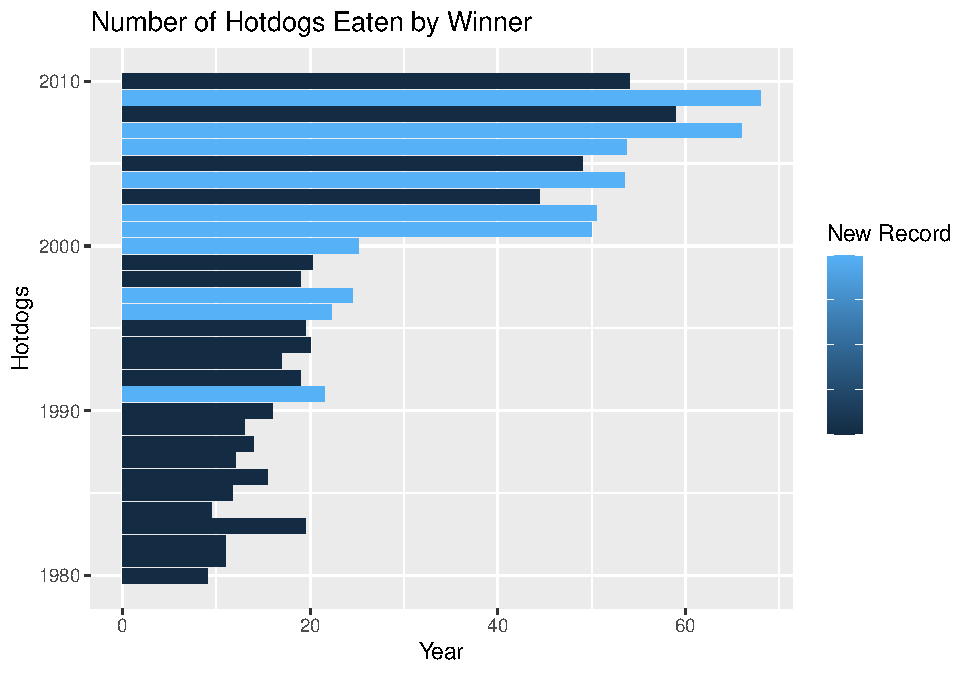
\includegraphics{C:/Users/Joshu/Desktop/Masters/DSC640/Week1/week1_files/figure-latex/bar-1.pdf}
\pagebreak

\hypertarget{stacked-bar-chart}{%
\subsection{Stacked Bar Chart}\label{stacked-bar-chart}}

\begin{Shaded}
\begin{Highlighting}[]
\CommentTok{\# Melt data set into proper format for plotting}
\NormalTok{meltObama }\OtherTok{\textless{}{-}} \FunctionTok{melt}\NormalTok{(thanksObama)}
\end{Highlighting}
\end{Shaded}

\begin{verbatim}
## Using Issue as id variables
\end{verbatim}

\begin{Shaded}
\begin{Highlighting}[]
\CommentTok{\# Plot stacked bar chart}
\FunctionTok{ggplot}\NormalTok{(meltObama, }\FunctionTok{aes}\NormalTok{(}\AttributeTok{x=}\NormalTok{Issue, }\AttributeTok{y=}\NormalTok{value, }\AttributeTok{fill=}\NormalTok{variable)) }\SpecialCharTok{+} 
  \FunctionTok{geom\_bar}\NormalTok{(}\AttributeTok{stat=}\StringTok{"identity"}\NormalTok{) }\SpecialCharTok{+} \FunctionTok{coord\_flip}\NormalTok{() }\SpecialCharTok{+} 
  \FunctionTok{ggtitle}\NormalTok{(}\StringTok{"Obama\textquotesingle{}s Approval Ratings by Issue"}\NormalTok{) }\SpecialCharTok{+} 
  \FunctionTok{labs}\NormalTok{(}\AttributeTok{y=}\StringTok{"Percent of Response"}\NormalTok{, }\AttributeTok{x=}\StringTok{"Political Issue"}\NormalTok{) }\SpecialCharTok{+} 
  \FunctionTok{labs}\NormalTok{(}\AttributeTok{fill=}\StringTok{"Response"}\NormalTok{)}
\end{Highlighting}
\end{Shaded}

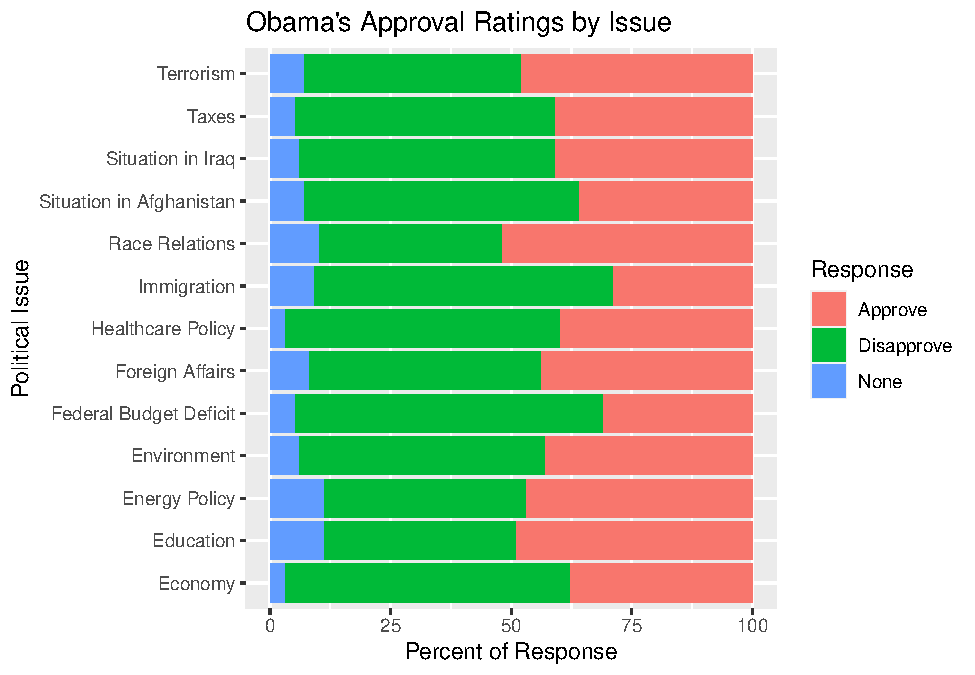
\includegraphics{C:/Users/Joshu/Desktop/Masters/DSC640/Week1/week1_files/figure-latex/stacked-1.pdf}
\pagebreak

\hypertarget{pie-chart}{%
\subsection{Pie Chart}\label{pie-chart}}

\begin{Shaded}
\begin{Highlighting}[]
\CommentTok{\# Convert data to table}
\NormalTok{mytable }\OtherTok{\textless{}{-}} \FunctionTok{table}\NormalTok{(dogDF}\SpecialCharTok{$}\NormalTok{Country, }\AttributeTok{dnn =} \FunctionTok{list}\NormalTok{(}\StringTok{"Country"}\NormalTok{))}
\CommentTok{\# Set up chart labels}
\NormalTok{lbls }\OtherTok{\textless{}{-}} \FunctionTok{paste}\NormalTok{(}\FunctionTok{names}\NormalTok{(mytable), }\StringTok{"}\SpecialCharTok{\textbackslash{}n}\StringTok{"}\NormalTok{, mytable, }\AttributeTok{sep=}\StringTok{""}\NormalTok{)}
\CommentTok{\# Plot pie chart}
\FunctionTok{pie}\NormalTok{(mytable, }\AttributeTok{labels =}\NormalTok{ lbls, }
    \AttributeTok{main =} \StringTok{"Hotdog Eating Competition: Wins by Country"}\NormalTok{)}
\end{Highlighting}
\end{Shaded}

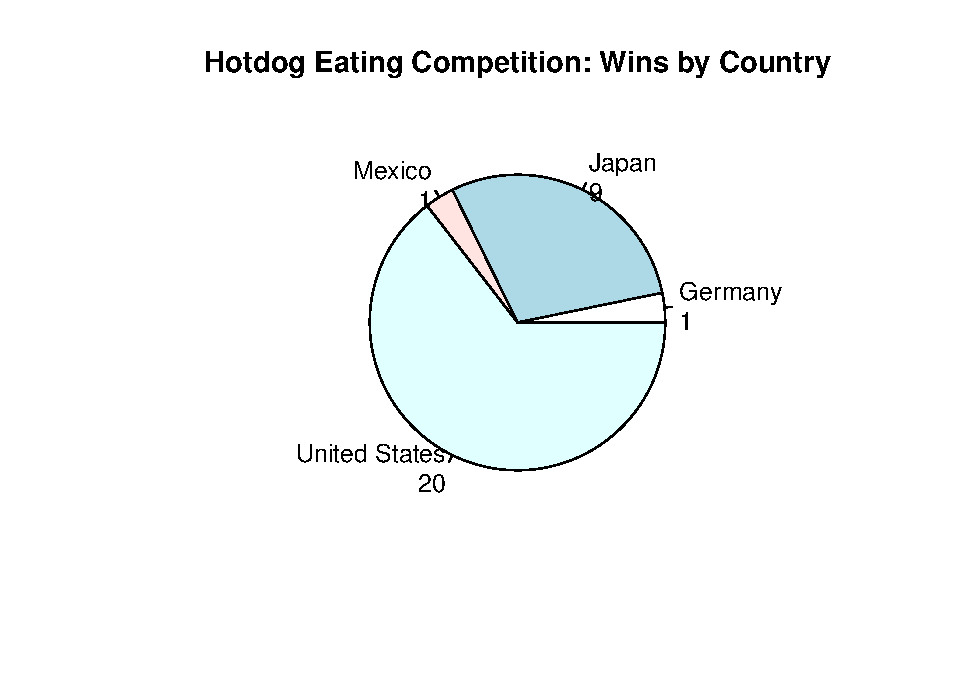
\includegraphics{C:/Users/Joshu/Desktop/Masters/DSC640/Week1/week1_files/figure-latex/pie-1.pdf}
\pagebreak

\hypertarget{donut-chart}{%
\subsection{Donut Chart}\label{donut-chart}}

\begin{Shaded}
\begin{Highlighting}[]
\CommentTok{\# Compute percentages}
\NormalTok{winsDF }\OtherTok{\textless{}{-}} \FunctionTok{as.data.frame}\NormalTok{(mytable, }\AttributeTok{responseName =} \StringTok{"Wins"}\NormalTok{)}
\NormalTok{winsDF}\SpecialCharTok{$}\NormalTok{fraction }\OtherTok{\textless{}{-}}\NormalTok{ winsDF}\SpecialCharTok{$}\NormalTok{Wins }\SpecialCharTok{/} \FunctionTok{sum}\NormalTok{(winsDF}\SpecialCharTok{$}\NormalTok{Wins)}
\CommentTok{\# Compute the cumulative percentages}
\NormalTok{winsDF}\SpecialCharTok{$}\NormalTok{ymax }\OtherTok{\textless{}{-}} \FunctionTok{cumsum}\NormalTok{(winsDF}\SpecialCharTok{$}\NormalTok{fraction)}
\CommentTok{\# Compute the bottom of each rectangle}
\NormalTok{winsDF}\SpecialCharTok{$}\NormalTok{ymin }\OtherTok{\textless{}{-}} \FunctionTok{c}\NormalTok{(}\DecValTok{0}\NormalTok{, }\FunctionTok{head}\NormalTok{(winsDF}\SpecialCharTok{$}\NormalTok{ymax, }\AttributeTok{n=}\SpecialCharTok{{-}}\DecValTok{1}\NormalTok{))}
\CommentTok{\# Compute label position}
\NormalTok{winsDF}\SpecialCharTok{$}\NormalTok{labelPosition }\OtherTok{\textless{}{-}}\NormalTok{ (winsDF}\SpecialCharTok{$}\NormalTok{ymax }\SpecialCharTok{+}\NormalTok{ winsDF}\SpecialCharTok{$}\NormalTok{ymin) }\SpecialCharTok{/} \DecValTok{2}
\CommentTok{\# Plot the donut chart}
\FunctionTok{ggplot}\NormalTok{(winsDF, }\FunctionTok{aes}\NormalTok{(}\AttributeTok{ymax=}\NormalTok{ymax, }\AttributeTok{ymin=}\NormalTok{ymin, }\AttributeTok{xmax=}\DecValTok{4}\NormalTok{, }\AttributeTok{xmin=}\DecValTok{3}\NormalTok{, }\AttributeTok{fill=}\NormalTok{Country)) }\SpecialCharTok{+} 
  \FunctionTok{geom\_rect}\NormalTok{() }\SpecialCharTok{+} 
  \FunctionTok{geom\_text}\NormalTok{(}\AttributeTok{x=}\FloatTok{3.5}\NormalTok{, }\FunctionTok{aes}\NormalTok{(}\AttributeTok{y=}\NormalTok{labelPosition, }\AttributeTok{label=}\NormalTok{Wins), }\AttributeTok{size=}\DecValTok{5}\NormalTok{) }\SpecialCharTok{+}
  \FunctionTok{coord\_polar}\NormalTok{(}\AttributeTok{theta =} \StringTok{\textquotesingle{}y\textquotesingle{}}\NormalTok{) }\SpecialCharTok{+}
  \FunctionTok{xlim}\NormalTok{(}\FunctionTok{c}\NormalTok{(}\DecValTok{2}\NormalTok{, }\DecValTok{4}\NormalTok{)) }\SpecialCharTok{+}
  \FunctionTok{theme\_void}\NormalTok{() }\SpecialCharTok{+}
  \FunctionTok{ggtitle}\NormalTok{(}\StringTok{"Hotdog Eating Competition: Wins by Country"}\NormalTok{)}
\end{Highlighting}
\end{Shaded}

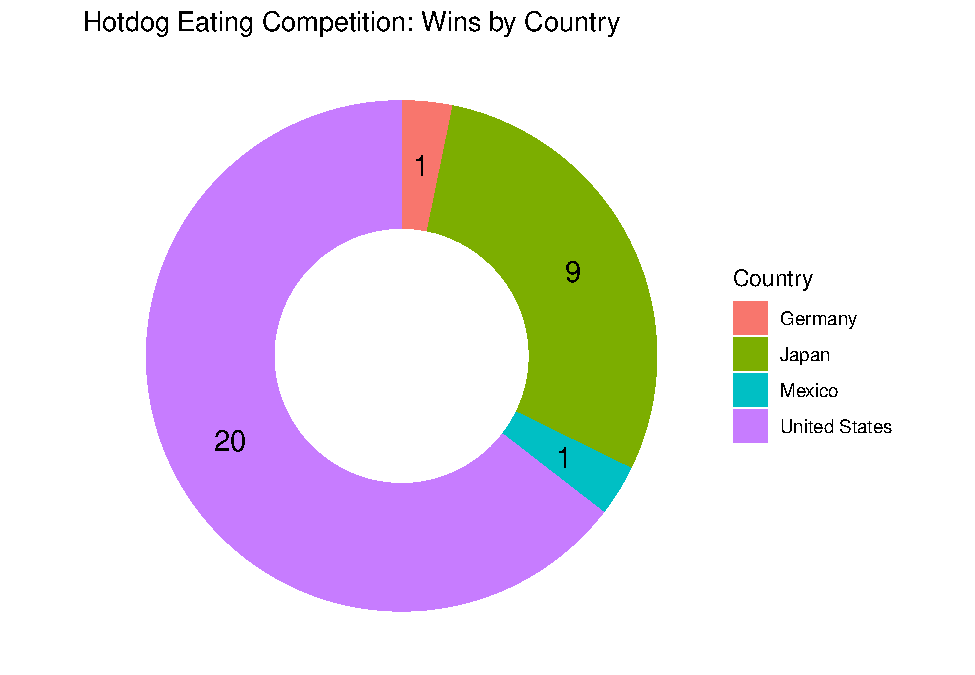
\includegraphics{C:/Users/Joshu/Desktop/Masters/DSC640/Week1/week1_files/figure-latex/donut-1.pdf}

\end{document}
